\documentclass[DaoFP]{subfiles}
\begin{document}
\setcounter{chapter}{16}

\chapter{Ends and Coends}

\section{Profunctors}

In the rarified air of category theory we encounter patterns that are so far removed from their origins that we have problems visualizing them. It doesn't help that the more abstract a pattern gets the more dissimilar the concrete examples of it are. 

An arrow from $A$ to $B$ is relatively easy to visualize. We have a very familiar model for it: a function that consumes elements of $A$ and produces elements of $B$. A hom-set is a collection of such arrows. 

A functor is an arrow between categories. It consumes objects and arrows from one category and produces objects and arrows from another. We can think of it a recipe for building such objects and arrows from materials provided by the source category. In particular, we  often think of an endofunctor as a container of building materials.

A profunctor maps a pair of objects $\langle A, B \rangle$ to a set $P\langle A, B \rangle$ and a pair of arrows:
\[ \langle f \colon S \to A, g \colon B \to T \rangle \]
to a function:
\[ P\langle f, g \rangle \colon P\langle A, B \rangle \to P\langle S, T \rangle\]

A profunctor is an abstraction that combines elements of many other abstractions. Since it's a functor $ \mathcal{C}^{op} \times  \mathcal{C} \to \mathbf{Set}$, we can think of it as constructing a set from a pair of objects and a function from a pair of arrows (one going in the opposite direction). This doesn't help our imagination though.

Fortunately, we have a good model for a profunctor: the hom-functor. The set of arrows between two objects behaves like a profunctor when you vary the objects. It also makes sense that there is a difference between varying the source and the target of the hom-set. 

We can, therefore, think of an arbitrary profunctor as generalizing a hom-functor. A profunctor provides additional bridges between objects. 

There is, however one big difference between an element of the hom-set $ \mathcal{C}(A, B)$ and an element of the set $P\langle A, B \rangle$. Elements of hom-sets are arrows, and arrows can be composed. It's not immediately obvious how to compose profunctors. 

However, the lifting of arrows by a profunctor can be seen as generalizing composition---just not between profuctors, but between hom-sets and profunctors. For instance, we can precompose $P \langle A, B \rangle$ with an arrow $f \colon S \to A$ to obtain $P \langle S, B \rangle$:
\[ P\langle f, id_B \rangle \colon P \langle A, B \rangle \to P \langle S, B \rangle \]
Similarly, we can postcompose it with $g \colon B \to T$:
\[ P \langle id_A, g \rangle \colon P \langle A, B \rangle \to P \langle A, T \rangle \]
This kind of heterogenous composition takes a composable pair consisting of an arrow and an element of a profunctor and produces an element of a profunctor.

In general, a profunctor can be extended this way on both sides by lifting a pair of arrows:

\[
 \begin{tikzcd}
  & S
  \arrow[r, bend left, dashed, blue, "f"]
 & A
 \arrow[r, bend right, "P"]
 & B
  \arrow[r, bend left, dashed, blue, "g"]
 &  T
  \end{tikzcd}
\]

\subsection{Collages}

There is no reason to restrict a profunctor to a single category. We can easily define a profunctor between two categories as a functor $ P \colon \mathcal{C}^{op} \times  \mathcal{D} \to \mathbf{Set}$. Such a profunctor can be used to glue two categories together by generating the missing hom-sets from the objects in $\mathcal{C}$ to the objects in $\mathcal{D}$. 

A collage (or a \index{cograph}cograph) of two categories $\mathcal{C}$ and $\mathcal{D}$ is a category whose objects are objects from both categories (a disjoint union). A hom-set between two objects $X$ and $Y$ is either a hom-set in $\mathcal{C}$, if both objects are in $\mathcal{C}$; a hom-set in $\mathcal{D}$, if both are in $\mathcal{D}$; or the set $P \langle X, Y\rangle$ if $X$ is in $\mathcal{C}$ and $Y$ is in $\mathcal{D}$. Otherwise the hom-set is empty. 

Composition of morphisms is the usual composition, except if one of the morphisms is an element of $P \langle X, Y \rangle$. In that case we use the profunctor to lift the morphism we're trying to compose. 

It's easy to see that a collage is indeed a category. The new morphisms that go between the two sides of the collage are sometimes called heteromorphisms. They can only go from $\mathcal{C}$ to $\mathcal{D}$, never the other way around. 

Seen this way, a profunctor $ \mathcal{C}^{op} \times  \mathcal{C} \to \mathbf{Set}$ should really be called an endo-profunctor. It defines a collage of $\mathcal{C}$ with itself.

\begin{exercise}
Show that there is a functor from a collage of two categories to a stick-figure ``walking arrow'' category that has two objects and one arrow between them (and two identity arrows).
\end{exercise}
\begin{exercise}
Show that, if there is a functor from $\mathcal{C}$ to the walking arrow category then $\mathcal{C}$ can be split into a collage of two categories. 
\end{exercise}

\subsection{Profunctors as relations}

Under a microscope, a profunctor looks like a hom-functor, and the elements of the set $P \langle A, B \rangle$ look like individual arrows. But when we zoom out, we can view a profunctor as a relation between objects. These are not the usual relations; they are \emph{proof-relevant} relations.

To understand this concept better, let's consider a regular functor $F \colon \mathcal{C} \to \mathbf{Set}$ (in other words, a co-presheaf). One way to interpret it is to say that it definines a subset of objects of $\mathcal{C}$, namely those objects that are mapped to non-empty sets. Every element of $F A$ is then treated as a proof that $A$ is a member of this subset. If, on the other hand, $F A$ is an empty set, then $A$ is not a member of the subset.

We can apply the same interpretation to profunctors. If the set $P \langle A, B \rangle$ is empty, we say that $B$ is not related to $A$. If it's not empty, we say that each element of the set represents a proof that $B$ is related to $A$. We can then treat a profunctor as a proof-relevant relation. 

Notice that we don't assume anything about this relation. It doesn't have to be reflexive, as it's possible for $P \langle A, A \rangle$ to be empty (in fact, $P \langle A, A \rangle$ makes sense only for endo-profunctors). It doesn't have to be symmetric either.

Since the hom-functor is an example of an (endo-) profunctor, this interpretation lets us view the hom-functor in a new light, as a built-in proof-relevant relation between objects in a category. If there's an arrow between two objects, they are related. Notice that this relation is reflexive, since $\mathcal{C}(A, A)$ is never empty: at the very least, it contains the identity morphism. 

Moreover, as we've seen before, hom-functors interact with profunctors. If $A$ is related to $B$ through $P$, and the hom-sets $\mathcal{C}(S, A)$ and $\mathcal{D}(B, T)$ are non-empty, then automatically $S$ is related to $T$ through $P$. Profunctors are therefore proof-relevant relations that are compatible with the structure of the categories in which they operate.

We know how to compose a profunctor with hom-functors, but how would we compose two profunctors? We can get a clue from the composition of relations. 

Suppose that you want to charge your cellphone, but you don't have a charger. In order to connect you to a charger it's enough that you have a friend who owns a charger. Any friend will do. You compose the relation of having a friend with the relation of a person having a charger to get a relation of being able to charge your phone. The proof that you can charge your phone is a pair of proofs, one of friendship and one of the possession of a charger. 

In general, we say that two objects are related by the composite relation if there exists an object in the middle that is related to both of them. 

\subsection{Profunctor composition in Haskell}

Composition of relations can be translated to profunctor composition in Haskell. Let's first recall the definition of a profunctor:
\begin{haskell}
class Profunctor p where
  dimap :: (s -> a) -> (b -> t) -> (p a b -> p s t)
\end{haskell}

The key to understanding profunctor composition is that it requires the \emph{existence} of the object in the middle. For object $B$ to be related to object $A$ through the composite $P \diamond Q$ there has to exist an object $X$ that bridges the gap:
\[
 \begin{tikzcd}
  & A
  \arrow[r, bend left, blue, "Q"]
 & X
  \arrow[r, bend left, red, "P"]
 & B
  \end{tikzcd}
\]

This can be encoded in Haskell using an existential type. Given two profunctors \hask{p} and \hask{q}, their composition is a new profunctor \hask{Procompose p q}:
\begin{haskell}
data Procompose p q a b where
  Procompose ::  q a x -> p x b -> Procompose p q a b
\end{haskell}
We are using a \hask{GADT} to express the existential nature of the object \hask{x}. The two arguments to the constructor can be seen as a pair of proofs: one proves that \hask{x} is related to \hask{a}, and the other that \hask{b} is related to \hask{x}. This pair then constitutes the proof that \hask{b} is related to \hask{a}.

An existential type can be seen as a generalization of a sum type. We are summing over all possible types \hask{x}. Just like a finite sum can be constructed by injecting one of the alternatives (think of the two constructors of \hask{Either}), the existential type can be constructed by picking one particular type for \hask{x} and injecting it into the definition of \hask{Procompose}. 

Just as mapping out from a sum type requires a pair of function, one per each alternative; a mapping out from an existential type requires a family of functions, one per every type. Such a family, in Haskell, is given by a polymorphic function:
\begin{haskell}
mapOut :: Procompose p q a b -> (forall x. q a x -> p x b -> c) -> c
mapOut (Procompose qax pxb) f = (f qax pxb)
\end{haskell}

The composition of profunctors is again a profunctor, as can be seen from this instance:
\begin{haskell}
instance (Profunctor p, Profunctor q) => Profunctor (Procompose p q) 
  where
    dimap l r (Procompose qax pxb) = 
               Procompose (dimap l id qax) (dimap id r pxb)
\end{haskell}
This just says that you can extend the composite profunctor by extending the first one on the left and the second one on the right.

The fact that this definition of profunctor composition happens to work in Haskell is due to parametricity. The language constraints the types of profunctors in a way that makes it work. In general, though, taking a simple sum over intermediate objects would result in over-counting, so in category theory we have to compensate for that.

\section{Coends}

The over-counting in the naive definition of profunctor composition happens when two candidates for the object in the middle are connected by a morphism:
\[
 \begin{tikzcd}
  & A
  \arrow[r, bend left, blue, "Q"]
  &X
  \arrow[r, dashed, "f"]
 & Y
  \arrow[r, bend left, red, "P"]
 & B
  \end{tikzcd}
\]
We can either extend $Q$ on the right, by lifting $Q \langle id, f \rangle$, and use $Y$ as the middle object; or we can extend $P$ on the left, by lifting $P \langle f, id \rangle$, and use $X$ as the intermediary.

In order to avoid the double-counting, we have to tweak our definition of a sum type when applied to profunctors. The resulting construction is called a coend. 

First, let's re-formulate the problem. We are trying to sum over all objects $X$ in the cartesian product:
\[ P \langle A, X \rangle \times Q \langle X, B \rangle \]
The double-counting happens because we can open up the gap between the two profunctors, as long as there is a morphism that we can fit between them. So we are really looking at a more general product:
\[ P \langle A, X \rangle \times Q \langle Y, B \rangle \]
The important observation is that, if we fix the endpoints $A$ and $B$, this product is a profunctor in $\langle Y, X \rangle$. This is easily seen after a little rearrangement (up to isomorphism):
\[ Q \langle Y, B \rangle \times P \langle A, X \rangle \]
We are interested in the sum of the diagonal parts of this profunctor, that is when $X$ is equal to $Y$. 

So let's see how we would go about defining the sum of all diagonal entries of a general profunctor $P$. The sum is defined by injections; in this case, one per every object in the category. Here just two of them are shown:
\[
 \begin{tikzcd}
 P \langle Y, Y \rangle
 \arrow[dr, "i_Y"']
 \arrow[rr, dash, dotted]
 &&P \langle X, X \rangle
 \arrow[dl, "i_X"]
 \\
 &C
 \end{tikzcd}
\]

If we were defining a sum, we'd make it a universal set equipped with such injections. But because we are dealing with profunctors, we want to identify the injections that are related by ``extending'' a common ancestor (here, $P \langle Y, X \rangle$). We want the following diagram to commute, whenever there is a connecting morphism $f\colon X \to Y$:

\[
 \begin{tikzcd}
 &P \langle Y, X \rangle
 \arrow[ld, "{P \langle id, f \rangle}"']
 \arrow[rd, "{P \langle f, id \rangle}"]
 \\
 P \langle Y, Y \rangle
 \arrow[dr, "i_Y"']
 &&P \langle X, X \rangle
 \arrow[dl, "i_X"]
 \\
 &C
 \end{tikzcd}
\]
This diagram is called a \index{co-wedge}co-wedge, and its commuting condition is called the co-wedge condition. The universal co-wedge is called a coend.

Since a coend generalizes a sum to a potentially infinite domain, we write it using the integral sign, with the ``integration variable'' at the top:
\[ \int^{X\colon \mathcal{C}} P \langle X, X \rangle \]
Universality means that, whenever there is a set $C$ equipped with a family of functions $g_X \colon P \langle X, X \rangle \to C$ satisfying the co-wedge condition, there is a unique mapping out:
\[ h \colon \int^{X\colon \mathcal{C}} P \langle X, X \rangle \to C \]
that factorizes every $g_X$ through the injection $i_X$:
\[
 \begin{tikzcd}
 &P \langle Y, X \rangle
 \arrow[ld, "{P \langle id, f \rangle}"']
 \arrow[rd, "{P \langle f, id \rangle}"]
 \\
 P \langle Y, Y \rangle
 \arrow[dr, "i_Y"']
 \arrow[ddr, bend right,  "g_Y"']
 &&P \langle X, X \rangle
 \arrow[dl, "i_X"]
 \arrow[ddl, bend left,  "g_X"]
 \\
 &\int^X P \langle X, X \rangle
 \arrow[d, dashed, "h"]
 \\
 &C
 \end{tikzcd}
\]

Compare this with the definition of a sum of two objects:

\[
 \begin{tikzcd}
 A
 \arrow[dr,  bend left, "\text{Left}"']
 \arrow[ddr, bend right, "f"']
 && B
 \arrow[dl, bend right, "\text{Right}"]
 \arrow[ddl, bend left, "g"]
 \\
&A + B
\arrow[d, dashed, "h"]
\\
& C
 \end{tikzcd}
\]
Just like the sum was defined as a universal cospan, a coend is defined as a universal co-wedge. 

If you were to construct a coend, you would start with a sum (discriminated union) of all the sets $P \langle X, X \rangle$. Then you would identify the elements of this sum that satisfy the co-wedge condition. You'd identify the element $x \in P \langle X, X \rangle$ with the element $y \in P \langle Y, Y \rangle$ whenever there is an element $z  \in P \langle Y, X \rangle$ and a morphism $f \colon X \to Y$, such that:
\[ P \langle id, f \rangle (z) = y\]
and
\[ P \langle f, id \rangle (z) = x\]

Notice that, in a discrete category (which is just a set of objects with no arrows between them) the co-wedge condition is trivial (there are no $f$s other than identities), so a coend is just a straightforward sum (discriminated union) of the diagonal sets $P \langle X, X \rangle$.

\subsection{Profunctor composition using coends}

Equipped with the definition of a coend we can now formally define the composition of two profunctors:

\[ (P \diamond Q)\langle A, B \rangle = \int^{X\colon \mathcal{C}} Q \langle A, X \rangle \times P \langle X, B \rangle\]
Compare this with:
\begin{haskell}
data Procompose p q a b where
  Procompose ::  q a x -> p x b -> Procompose p q a b
\end{haskell}

The reason why, in Haskell, we don't have to worry about the co-wedge condition is analogous to the reason why all parametrically polymorphic functions automatically satisfy the naturality condition. A coend is defined using a family of injections; in Haskell they are all given as one polymorphic function:
\begin{haskell}
data Coend p where
  Coend ::  p x x -> Coend p
\end{haskell}

Coends introduce a new level of abstraction for dealing with profunctors. Calculations using coends usually take advantage of their mapping-out property. To define a mapping out of a coend to some set $C$:
\[ \int^X P \langle X, X \rangle \to C \]
 it's enough to define a family of functions from the diagonal entries of the profunctor to $C$:
 \[ g_X \colon P \langle X, X \rangle \to C \]
 You can get a lot of mileage from this trick, especially when combined with the Yoneda lemma. We'll see examples of this in what follows.

\begin{exercise}
Define a \hask{Profunctor} instance for the pair of profunctors:
\begin{haskell}
newtype ProPair q p a b x y = ProPair (q a y, p x b)
\end{haskell}
Hint: Keep the first four parameters fixed:
\begin{haskell}
instance (Profunctor p, Profunctor q) => Profunctor (ProPair q p a b)
\end{haskell}
\end{exercise}

\begin{exercise}
Profunctor composition can be expressed using a coend:
\begin{haskell}
newtype CoEndCompose p q a b = CoEndCompose (Coend (ProPair q p a b))
\end{haskell}
Define a \hask{Profunctor} instance for \hask{CoEndCompose}.
\end{exercise}


\section{Ends}

Just like a coend generalizes a sum of the diagonal elements of a profunctor; its dual, an end, generalizes the product. A product is defined by its projections, and so is an end. 

The generalization of a span that we used in the definition of a product would be a set $C$ with a family of projections, one per every object $X$ in the category:
\[ \pi_X \colon C \to P \langle X, X \rangle \]
The dual to a co-wedge is called a \index{wedge}wedge:
\[
 \begin{tikzcd}
 &C
 \arrow[ld, "\pi_X"']
 \arrow[rd, "\pi_Y"]
 \\
 P \langle X, X \rangle
 \arrow[dr, "{P \langle id, f \rangle}"']
 &&P \langle Y, Y \rangle
 \arrow[dl, "{P \langle f, id \rangle}"]
 \\
 & P \langle X, Y \rangle
 \end{tikzcd}
\]

You may think of constructing a set $C$ by first starting with a bigger set that is equipped with all the projections, and then restricting it to the elements that can be connected by way of lifting a morphism. 

The end is a universal wedge. We use the integral sign for it too, but with the ``integration variable'' at the bottom. 
\[ \int_X P \langle X, X \rangle \]

You might be wondering why integrals based on multiplication are rarely used in calculus. That's because we can use a logarithm to replace multiplication with addition. We don't have this luxury in category theory, so ends and coends are equally important.

An end is a set equipped with a family of functions (projections):
\[ \pi_A \colon \left( \int_X P \langle X, X \rangle \right) \to P \langle A, A \rangle \]
satisfying the wedge condition. It is universal among such sets; that is, for any other set $C$ equipped with a family of functions $g_X$, satisfying the wedge condition, there is a unique function $h$ that factorizes the family $g_X$ through the family $\pi_X$.
\[
 \begin{tikzcd}
 &C
 \arrow[ddl, bend right, "g_X"']
 \arrow[ddr, bend left, "g_Y"]
 \arrow[d, dashed, "h"]
 \\
 & \int_X P \langle X, X \rangle
 \arrow[ld, "\pi_X"']
 \arrow[rd, "\pi_Y"]
 \\
 P \langle X, X \rangle
 \arrow[dr, "{P \langle id, f \rangle}"']
 &&P \langle Y, Y \rangle
 \arrow[dl, "{P \langle f, id \rangle}"]
 \\
 & P \langle X, Y \rangle
 \end{tikzcd}
\]

If you were to construct this set, you'd start with a product of all $P \langle X, X \rangle$ for all objects in the category. 

Imagine for a moment using the singleton set $1$ in place of $C$. The family $g_X$ would select one element from each $P \langle X, X \rangle$. This would give you a giant tuple. You'd weed out most of these tuples, leaving only the ones that satisfy the wedge condition. 

Again, in Haskell, due to parametricity, the wedge condition is automatically satisfied, and the definition of an end for a profunctor $p$ simplifies to:

\begin{haskell}
type End p = forall x. p x x
\end{haskell}

The Haskell implementation of an \hask{End} doesn't showcase the fact that it is dual to a \hask{Coend}. This is because, at the time of this writing, Haskell doesn't have a built-in syntax for existential types. If it did, the \hask{Coend} would be implemented as:
\begin{haskell}
type Coend p = exists x. p x x
\end{haskell}

The existential/universal duality between a \hask{Coend} and an \hask{End} means that it's easy to construct a \hask{Coend}---all you need is to pick one type \hask{x} for which you have a value of the type \hask{p x x}. On the other end, to construct an \hask{End} you have to provide a whole family of values \hask{p x x}, one for every type \hask{x}. In other words, you need a polymorphic formula that is parameterized by \hask{x}. A definition of a polymorphic function is a canonical example of such a formula.


\subsection{Natural transformations as an end}

The most interesting application of an end is in concisely defining natural transformations. Consider two functors, $F$ and $G$, going between two categories  $\mathcal{B}$ and $\mathcal{C}$. A natural transformation between them is a family of arrows $\alpha_X$ in $\mathcal{C}$. You can think of it as picking one element $\alpha_X$ from each hom-set  $\mathcal{C} (F X, G X)$.
\[
 \begin{tikzcd}
 && F X
 \arrow[dd, "\alpha_X"]
 \\
 X
 \arrow[urr, dashed, "F"]
 \arrow[drr, dashed, "G"]
 \\
 && G X
 \end{tikzcd}
\]

The mapping  $\langle A, B \rangle \to \mathcal{C} (F A, G B)$ behaves as a profunctor. Its action on a pair of arrows $\langle f, g \rangle$ is a combination of pre- and post-composition of lifted arrows $(G g) \circ - \circ (F f)$. 

Indeed, an element of the set $ \mathcal{C} (F A, G B)$ is an arrow $h \colon F A \to G B$. We are trying to lift a pair of arrows $f \colon S \to A$ and $g \colon B \to T$. We can do it with a pair of arrows in $\mathcal{C}$: the first one is $F f \colon F S \to F A$, and the second one is $G g \colon G B \to G T$. The composition $G g \circ h \circ F f$ gives us the desired result $ F S \to G T$, which is an element of $\mathcal{C} (F S, G T)$.
\[ F S \xrightarrow{F f} F A \xrightarrow{h} G B \xrightarrow{G g} GT \]

The diagonal parts of this profunctor are good candidates for the components of a natural transformation. In fact, the end:
\[  \int_{X \colon  \mathcal{B}} \mathcal{C}(FX, GX) \]
defines a set of natural transformations from $F$ to $G$.

In Haskell, this is consistent with our earlier definition:
\begin{haskell}
type Natural f g = forall x. f x -> g x
\end{haskell}

In category theory, though, we have to check the wedge condition. Plugging in our profunctor, we get:

\[
 \begin{tikzcd}
 & \int_{X} \mathcal{C}(FX, GX)
 \arrow[ld, "\pi_A"']
 \arrow[rd, "\pi_B"]
 \\
  \mathcal{C} ( FA, GA )
 \arrow[dr, "{(Ff \, \circ \, -)}"']
 && \mathcal{C} \langle FB, GB \rangle
 \arrow[dl, "{(- \, \circ\, Gf)}"]
 \\
 &  \mathcal{C} ( FA, GB )
 \end{tikzcd}
\]

We can focus on a single element of the set $\int_{X} \mathcal{C}(FX, GX)$ by instantiating the universal condition for the singleton set:

\[
 \begin{tikzcd}
 & 1
 \arrow[d, dashed, "\alpha"]
\arrow[ddl, bend right, "\alpha_A"']
 \arrow[ddr, bend left, "\alpha_B"]
 \\
 & \int_{X \colon  \mathcal{B}} \mathcal{C}(FX, GX)
 \arrow[ld, "\pi_A"']
 \arrow[rd, "\pi_B"]
 \\
  \mathcal{C} ( FA, GA )
 \arrow[dr, "{(Ff \, \circ \, -)}"']
 && \mathcal{C} \langle FB, GB \rangle
 \arrow[dl, "{(- \, \circ\, Gf)}"]
 \\
 &  \mathcal{C} ( FA, GB )
 \end{tikzcd}
\]
It picks the component $\alpha_A$ from the hom-set $\mathcal{C} ( FA, GA )$ and the component $\alpha_B$ from $\mathcal{C} ( FB, GB )$. The wedge condition then boils down to:
\[ F f \circ \alpha_A = \alpha_B \circ G f \]
for any $f \colon A \to B$. This is exactly the naturality condition. So an element $\alpha$ of this end is indeed a natural transformation.

The set of natural transformations, or the hom-set in the functor category, is thus given by the end:
\[ [\mathcal{C}, \mathcal{D}] (F, G) \cong \int_{X \colon  \mathcal{B}} \mathcal{C}(FX, GX)\]

As we discussed earlier, to construct an \hask{End} we have to give it a whole family of values parameterized by types. Here, these values are the components of a polymorphic functions. 

\section{Continuity of the Hom-Functor}

In category theory, a functor is called continuous if it preserves limits (and co-continuous, if it preserves colimits). It means that, if you have a diagram in the source category then it doesn't matter if you first use the functor to map the diagram, and then take the limit; or take the limit in the source category, and then map this limit using the functor. 

The hom-functor is an example of a functor that is continuous in its second argument. Since a product is the simplest example of a limit, we should have:
\[ \mathcal{C}(X, A \times B) \cong \mathcal{C}(X, A) \times \mathcal{C}(X, B) \]
The left hand side applies the hom-functor to the product. The right hand side maps the diagram, a pair of objects, and takes the product in the target category, which for the hom-functor is $\mathbf{Set}$. The two sides are isomorphic by the universal property of the product: the mapping into the product is defined by a pair of mappings into the two objects. 

Continuity of the hom-functor in the first argument is reversed: it maps colimits to limits. Again, the simplest example of a colimit is the sum, so we have:
\[ \mathcal{C}(A + B, X) \cong \mathcal{C}(A, X) \times \mathcal{C}(B, X) \]
This follows from the universality of the sum: a mapping out of the sum is defined by a pair of mapping out of the two objects.

It can be shown that an end can be expressed as a limit, and a coend as a colimit. Therefore, by continuity of the hom-functor, we can always pull out the integral sign from inside a hom-set. By analogy with the product, we have the mapping-in formula for an end:
\[ \mathbf{Set}\left(X, \int_A P\langle A, A \rangle \right) \cong \int_A  \mathbf{Set}(X, P\langle A, A \rangle) \]
By analogy with the sum, we have a mapping-out formula for the coend:
\[ \mathbf{Set}\left( \int^A P\langle A, A \rangle , X\right) \cong \int_A  \mathbf{Set}(P\langle A, A \rangle, X) \]
Notice that, in both cases, the right-hand side is an end.

\section{Ninja Yoneda Lemma}

Having expressed natural transformations as an end, we can now rewrite the Yoneda lemma. This is the original formulation:
\[ [\mathcal{C}, \mathbf{Set}]( \mathcal{C}(A, -), F) \cong F A \]
$F$ is a (covariant) functor from $\mathcal{C}$ to $\mathbf{Set}$ (a co-presheaf) and so is the hom-functor $\mathcal{C}(A, -)$. 
Expressing the set of natural transformations as an end we get:
\[ \int_{X \colon \mathcal{C}} \mathbf{Set} (\mathcal{C}(A, X), FX) \cong FA \]

Similarly, we have the Yoneda lemma for a contravariant functor (a presheaf) $G$:
\[ \int_{X \colon \mathcal{C}} \mathbf{Set} (\mathcal{C}(X, A), GX) \cong GA \]

These versions of the Yoneda lemma, expressed in terms of ends, are often half-jokingly called ninja-Yoneda lemmas. The fact that the ``integration variable'' is explicit makes them somewhat easier to use in complex formulas.

There is also a dual set of ninja co-Yoneda lemmas that use coends instead. For a covariant functor, we have:
\[ \int^{X \colon \mathcal{C}} \mathcal{C}(X, A) \times F X \cong F A \]
and for the contravariant one we have:
\[ \int^{X \colon \mathcal{C}} \mathcal{C}(A, X) \times G X \cong G A \]

Physicists might notice the similarity of these formulas to integrals involving the Dirac delta function (actually, a distribution). This is why profunctors are sometimes called \index{distributors}distributors, following the adage that ``distributors are to functors as distributions are to functions.'' 

Yet another name for profunctors is \index{bimodule}``bimodules.''

The proof of the co-Yoneda lemma is quite instructive, as it uses a few common tricks. Most importantly, we rely on the corollary of the Yoneda lemma, which says that, if the mappings out from two objects to an arbitrary object are isomorphic, then the two objects themselves are isomorphic. We'll start, therefore, with such a mapping-out to an arbitrary set $S$:
\[ \mathbf{Set} \left(\int^{X \colon \mathcal{C}} \mathcal{C}(X, A) \times F X, S \right) \]
Using the co-continuity of the hom-functor, we can pull out the integral sign, replacing the coend with an end:
\[ \int_{X \colon \mathcal{C}} \mathbf{Set} \left( \mathcal{C}(X, A) \times F X, S \right) \]
Since the category of sets is cartesian closed, we can curry the product:
\[ \int_{X \colon \mathcal{C}} \mathbf{Set} \left( \mathcal{C}(X, A) , S^{FX} \right) \]
We can now use the Yoneda lemma to ``integrate over $X$.'' The result is $S^{FA}$. Finally, in $\mathbf{Set}$, the exponential object is isomorphic to the hom-set:
\[S^{FA} \cong \mathbf{Set}(F A, S)\]
Since $S$ was arbitrary, we conclude that:
\[ \int^{X \colon \mathcal{C}} \mathcal{C}(X, A) \times F X \cong F A \]

\begin{exercise}
Prove the contravariant version of the co-Yoneda lemma.
\end{exercise}

\subsection{Yoneda lemma in Haskell}

We've seen the Yoneda lemma implemented in Haskell. We can now rewrite it in terms of an end. We start by defining a profunctor that will go under the end. Its type constructor takes a functor \hask{f} and a type \hask{a} and generates a profunctor that's contravariant in \hask{x} and covariant in \hask{y}:
\begin{haskell}
data Yo f a x y = Yo ((a -> x) -> f y)
\end{haskell}
The Yoneda lemma establishes the isomorphism between the end over this profunctor and the type obtained by acting with the functor  \hask{f} on \hask{a}. This isomorphism is witnessed by a pair of functions:
\begin{haskell}
yoneda :: Functor f => End (Yo f a) -> f a
yoneda (Yo g) = g id

yoneda_1 :: Functor f => f a -> End (Yo f a)
yoneda_1 fa = Yo (\h -> fmap h fa)
\end{haskell}

Similarly, the co-Yoneda lemma uses a coend over the following profunctor:
\begin{haskell}
data CoY f a x y = CoY (x -> a) (f y)
\end{haskell}
The isomorphism is witnessed by a pair of functions. The first one says that if you have a function \hask{x -> a} and a functorful of \hask{x} then you can make a functorful of \hask{a} using the \hask{fmap}:
\begin{haskell}
coyoneda :: Functor f => Coend (CoY f a) -> f a
coyoneda (Coend (CoY g fa)) = fmap g fa
\end{haskell}
You can do it without knowing anything about the existential type \hask{x}.

The second says that if you have a functorful of \hask{a} then you can create a coend by injecting it (together with the identity function) into the existential type:
\begin{haskell}
coyoneda_1 :: Functor f => f a -> Coend (CoY f a)
coyoneda_1 fa = Coend (CoY id fa)
\end{haskell}


\section{The Bicategory of Profunctors}

Since we know how to compose profunctors using coends, the question arises: is there a category in which they serve as morphisms? The answer is yes, as long as we relax the rules a bit. The problem is that the categorical laws for profunctor composition are satisfied up to isomorphism. 

For instance, we can try to show associativity of profunctor composition. We start with:
\[ ((P \diamond Q) \diamond R) \langle S, T \rangle = \int^B \left( \int^A P \langle S, A \rangle \times Q \langle A, B \rangle \right) \times R \langle B,  T \rangle \]
and, after a few transformations, arrive at:
\[ (P \diamond (Q \diamond R)) \langle S, T \rangle =  \int^A P \langle S, A \rangle \times \left( \int^B Q \langle A, B \rangle \times R \langle B,  T \rangle \right) \]
We use the associativity of the product and the fact that we can switch the order of coends (it's called the \index{Fubini theorem} Fubini theorem). Both are true only up to isomorphism. We don't get associativity ``on the nose.''

The identity profunctor turns out to be the hom-functor, which can be written symbolically as $\mathcal{C}(-, =)$, with placeholders for both arguments. For instance:
\[ \left( \mathcal{C}(-, =) \diamond P \right) \langle S, T \rangle \cong \int^A  \mathcal{C}(S, A) \times P \langle A, T \rangle = P \langle S, T \rangle \]
This is the consequence of the (contravariant) ninja co-Yoneda lemma, which is also an isomorphism---not an equality.

A category in which categorical laws are satisfied up to isomorphism is called a bicategory. Notice that such a category must be equipped with 2-cells---morphisms between morphisms, which we've seen in the definition of a 2-category. We need those in order to be able to define isomorphisms between 1-cells. 

A bicategory $\mathbf{Prof}$ has (small) categories as objects, profunctors as 1-cells, and natural transformations as 2-cells. 

Since profunctors are functors $\mathcal{C}^{op} \times  \mathcal{D} \to \mathbf{Set}$, the standard definition of natural transformations between them applies. It's a family of functions parameterized by objects of $\mathcal{C}^{op} \times  \mathcal{D}$, which are themseves pairs of objects. 

The naturality condition for a transformation $\alpha_{\langle A, B \rangle}$ between two profunctors $P$ and $Q$ takes the form:
\[
 \begin{tikzcd}
 &P \langle A, B \rangle
 \arrow[ld, "{\alpha_{\langle A, B \rangle}}"']
 \arrow[rd, "{P \langle f, g \rangle}"]
 \\
 Q \langle A, B \rangle
 \arrow[dr, "{Q \langle f, g \rangle}"']
 &&P \langle S, T \rangle
 \arrow[dl, "{\alpha_{\langle S, T \rangle}}"]
 \\
 & Q \langle S, T \rangle
 \end{tikzcd}
\]
for every pair of arrows:
\[ \langle f \colon S \to A, g \colon B \to T \rangle \]

\section{Existential Lens}

The first rule of category-theory club is that you don't talk about the internals of objects.

The second rule of category-theory club is that, if you have to talk about the internals of objects, use arrows only.

\subsection{Existential lens in Haskell}

What does it mean for an object to be a composite---to have parts? At the very minimum, you should be able to retrieve a part of such an object. Even better if you can replace that part with a new one. This pretty much defines a lens:
\begin{haskell}
get :: s -> a
set :: s -> a -> s
\end{haskell}
Here, \hask{get} extracts the part \hask{a} from the whole \hask{s}, and \hask{set} replaces that part with a new \hask{a}. Lens laws help to reinforce this picture. And it's all done in terms of arrows. 

Another way of describing a composite object is to say that it can be split into a focus and a residue. The trick is that, although we want to know what type the focus is, we don't care about the type of the residue. All we need to know about the residue is that it can be combined with the focus to recreate the whole object. 

In Haskell, we would express this idea using an existential type:
\begin{haskell}
data Lens s a where
    Lens :: (s -> (c, a), (c, a) -> s) -> Lens s a
\end{haskell}
This tells us that there exists some unspecified type \hask{c} such that \hask{s} can be split into, and reconstructed from, a product \hask{(c, a)}. 

\[
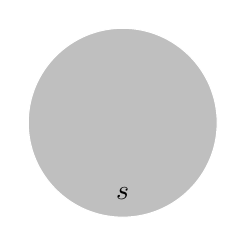
\begin{tikzpicture}
\filldraw[fill=gray!50, draw=white] (0, 0) circle (1.2);
\node at (0, -0.9) {$s$};
\end{tikzpicture}
\hspace{20pt}
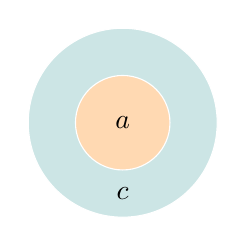
\begin{tikzpicture}
\filldraw[fill=blue!50!green!20, draw=white] (0, 0) circle (1.2);
\filldraw[fill=orange!30, draw=white] (0, 0) circle (0.6);
\node at (0, 0) {$a$};
\node at (0, -0.9) {$c$};
\end{tikzpicture}
\]



The \hask{get}/\hask{set} version of the lens can be derived from this existential form.
\begin{haskell}
toGet :: Lens s a -> (s -> a)
toGet (Lens (l, r)) = snd . l

toSet :: Lens s a -> (s -> a -> s)
toSet (Lens (l, r)) s a = r (fst (l s), a)
\end{haskell}

Notice that we don't need to know anything about the type of the residue. We take advantage of the fact that the existential lens contains both the producer and the consumer of \hask{c}.

It's impossible to extract a ``naked'' residue, as witnessed by the fact that the following code doesn't compile:
\begin{haskell}
getResidue :: Lens s a -> c
getResidue (Lens (l, r)) = fst . l
\end{haskell}

\subsection{Existential lens in category theory}

We can easily translate the new definition of the lens to category theory by expressing the existential type as a coend:
\[ \int^{C} \mathcal{C}(S, C \times A) \times  \mathcal{C}(C \times A, S) \]
In fact, we can generalize it to a type-changing lens, in which the focus $A$ can be replaced with a new focus of a different type $B$. Replacing $A$ with $B$ will produce a new composite object $T$:
\[
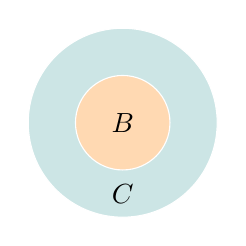
\begin{tikzpicture}
\filldraw[fill=blue!50!green!20, draw=white] (0, 0) circle (1.2);
\filldraw[fill=orange!30, draw=white] (0, 0) circle (0.6);
\node at (0, 0) {$B$};
\node at (0, -0.9) {$C$};
\end{tikzpicture}
\hspace{20pt}
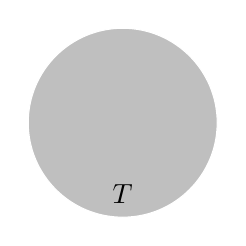
\begin{tikzpicture}
\filldraw[fill=gray!50, draw=white] (0, 0) circle (1.2);
\node at (0, -0.9) {$T$};
\end{tikzpicture}
\]

The lens is now parameterized by two pairs of objects: $\langle S, T\rangle$ for the outer ones, and $ \langle A, B \rangle$ for the inner ones. The existential residue $C$ remains hidden:
\[ \mathcal{L}\langle S, T\rangle \langle A, B \rangle = \int^{C} \mathcal{C}(S, C \times A) \times  \mathcal{C}(C \times B, T) \]
The product under the coend is the diagonal part of the profunctor that is covariant in $Y$ and contravariant in $X$:
\[ \mathcal{C}(S, Y \times A) \times  \mathcal{C}(X \times B, T) \]
\begin{exercise}
Show that:
\[ \mathcal{C}(S, Y \times A) \times  \mathcal{C}(X \times B, T) \]
is a profunctor in $\langle X, Y\rangle$.
\end{exercise}


\subsection{Type-changing lens in Haskell}
In Haskell, we can define a type-changing lens as the existential type:
\begin{haskell}
data Lens s t a b where
 Lens :: (s -> (c, a)) -> ((c, b) -> t) -> Lens s t a b
\end{haskell}
As before, we can use it to get and set the focus:
\begin{haskell}
toGet :: Lens s t a b -> (s -> a)
toGet (Lens l r) = snd . l

toSet :: Lens s t a b -> (s -> b -> t)
toSet (Lens l r) s a = r (fst (l s), a)
\end{haskell}

The simplest example of a lens acts on a product. It can extract or replace one component of the product, treating the other as the residue. In Haskell, we'd implement it as:
\begin{haskell}
prodLens :: Lens (c, a) (c, b) a b
prodLens = Lens id id
\end{haskell}
Here, the type of the whole is a product \hask{(c, a)}. When we replace \hask{a} with \hask{b} we end up with the target type \hask{(c, b)}.

\subsection{Lens composition}

The main advantage of using lenses is that they compose. A composition of two lenses lets us zoom in on a subcomponent of a component. 

Suppose that we start with a lens that lets us access and modify the focus described by the pair \hask{a} and \hask{b}. This focus is part of a whole described by the pair \hask{s} and \hask{t}. We also have a lens that can access the focus of \hask{a'} and \hask{b'} inside the whole of \hask{a} and \hask{b}. We can now construct a new lens that can access \hask{a'} and \hask{b'} inside of \hask{s} and \hask{t}. The trick is to realize that we can take as the new residue a product of the two residues:
\[
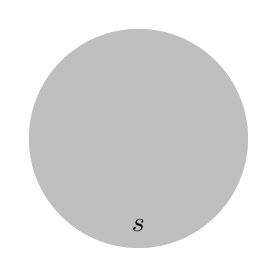
\begin{tikzpicture}
\filldraw[fill=gray!50, draw=white] (0, 0) circle (1.4);
\node at (0, -1.1) {$s$};
\end{tikzpicture}
\hspace{20pt}
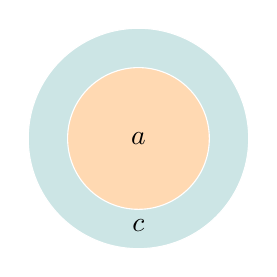
\begin{tikzpicture}
\filldraw[fill=blue!50!green!20, draw=white] (0, 0) circle (1.4);
\filldraw[fill=orange!30, draw=white] (0, 0) circle (0.9);
\node at (0, 0) {$a$};
\node at (0, -1.1) {$c$};
\end{tikzpicture}
\hspace{20pt}
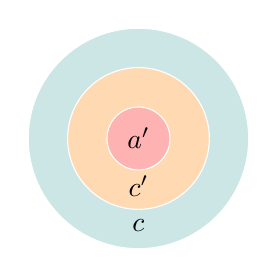
\begin{tikzpicture}
\filldraw[fill=blue!50!green!20, draw=white] (0, 0) circle (1.4);
\filldraw[fill=orange!30, draw=white] (0, 0) circle (0.9);
\filldraw[fill=red!30, draw=white] (0, 0) circle (0.4);
\node at (0, 0) {$a'$};
\node at (0, -0.6) {$c'$};
\node at (0, -1.1) {$c$};
\end{tikzpicture}
\]

\[
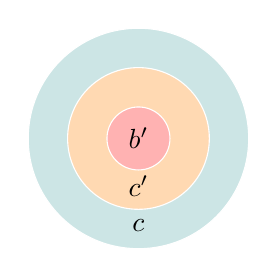
\begin{tikzpicture}
\filldraw[fill=blue!50!green!20, draw=white] (0, 0) circle (1.4);
\filldraw[fill=orange!30, draw=white] (0, 0) circle (0.9);
\filldraw[fill=red!30, draw=white] (0, 0) circle (0.4);
\node at (0, 0) {$b'$};
\node at (0, -0.6) {$c'$};
\node at (0, -1.1) {$c$};
\end{tikzpicture}
\hspace{20pt}
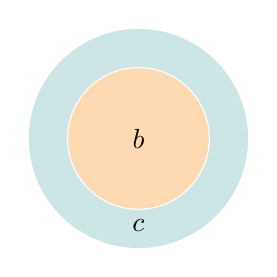
\begin{tikzpicture}
\filldraw[fill=blue!50!green!20, draw=white] (0, 0) circle (1.4);
\filldraw[fill=orange!30, draw=white] (0, 0) circle (0.9);
\node at (0, 0) {$b$};
\node at (0, -1.1) {$c$};
\end{tikzpicture}
\hspace{20pt}
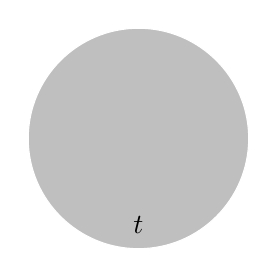
\begin{tikzpicture}
\filldraw[fill=gray!50, draw=white] (0, 0) circle (1.4);
\node at (0, -1.1) {$t$};
\end{tikzpicture}
\]



\begin{haskell}
compLens :: Lens a b a' b' -> Lens s t a b -> Lens s t a' b'
compLens (Lens l2 r2) (Lens l1 r1) = Lens l3 r3
  where l3 = assoc' . bimap id l2  . l1
        r3 = r1 . bimap id r2 . assoc
\end{haskell}
The left mapping in the new lens is given by the following composite:
\[ s \xrightarrow{l_1} (c, a)   \xrightarrow{(id, l_2)} (c, (c', a'))  \xrightarrow{assoc'} ((c, c'), a')\]
and the right mapping is given by:
\[ ((c, c'), b') \xrightarrow{assoc}  (c, (c', b')) \xrightarrow{(id, r_2)} (c, b) \xrightarrow{r_1} t \]

We have used the associativity and functoriality of the product:
\begin{haskell}
assoc :: ((c, c'), b') -> (c, (c', b'))
assoc ((c, c'), b') = (c, (c', b'))

assoc' :: (c, (c', a')) -> ((c, c'), a')
assoc' (c, (c', a')) = ((c, c'), a')

instance Bifunctor (,) where
  bimap f g (a, b) = (f a, g b)
\end{haskell}

As an example, let's compose two product lenses:
\begin{haskell}
l3 :: Lens (c, (c', a')) (c, (c', b')) a' b'
l3 = compLens prodLens prodLens
\end{haskell}
and apply it to a nested product:
\begin{haskell}
x :: (String, (Bool, Int))
x = ("Outer", (True, 42))
\end{haskell}
Our composite lens lets us not only retrieve the innermost component:
\begin{haskell}
toGet l3 x
> 42
\end{haskell}
but also replace it with a value of a different type (here, \hask{Char}):
\begin{haskell}
toSet l3 x 'z'
> ("Outer",(True,'z'))
\end{haskell}

\subsection{Category of lenses}

Since lenses can be composed, you might be wondering if there is a category in which lenses serve as hom-sets. 

Indeed, there is a category $\mathbf{Lens}$ whose objects are pairs of objects in $\mathcal{C}$, and arrows from $\langle S, T\rangle$ to $ \langle A, B \rangle$ are elements of  $\mathcal{L} \langle S, T\rangle \langle A, B \rangle$.

The formula for the composition of existential lenses is too complicated to be useful in practice. In the next chapter we'll see an alternative representation of lenses using Tambara modules, in which composition of lenses is just a composition of functions.

\section{Lenses and Fibrations}

There is an alternative view of lenses using the language of fiber bundles. A projection $p$ that defines a fibration can be seen as ``decomposing'' the bundle $E$ into fibers. 

In this view, $p$ plays the role of \hask{get}:
\[ p \colon E \to B \]
The base $B$ represents the type of the focus. 

The other part of the lens, \hask{set}, is a mapping: 
\[ q \colon E \times B \to E \]
\subsection{Transport law}

We interpret $q$ as ``transporting'' an element of the bundle to a new fiber because of the get/set lens law, or the \emph{transport} law:
\begin{haskell}
get (set s a) = a
\end{haskell}
We say that $q(s, a)$ transports $s$ to a new fiber over $a$:

\[
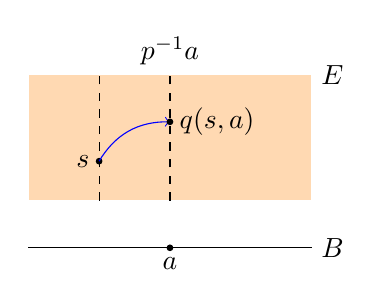
\begin{tikzpicture}

\def\yb{0}; % base
\def\yfb{0.6}; % fiber bottom
\def\yfs{1.1}; % s
\def\yfss{1.6}; % s'
\def\yft{2.2}; % fiber top

\def\dx{0.9};

\def\xbl{0};
\def\xbm{\xbl + \dx};
\def\xbmr{\xbl + 2*\dx};
\def\xbr{\xbl + 4*\dx};


\filldraw[fill=orange!30, draw=white] (\xbl, \yfb) rectangle (\xbr, \yft);

\draw (\xbl, \yb) -- (\xbr, \yb);

\draw[dashed] (\xbm, \yfb) -- (\xbm, \yft); %fiber
\draw[dashed] (\xbmr, \yfb) -- (\xbmr, \yft); %fiber

\filldraw[black] (\xbm, \yfs) circle (1 pt);
\node[left] at (\xbm, \yfs) {$s$};
\draw[blue] (\xbm, \yfs) edge[->, bend left] (\xbmr, \yfss);
\filldraw[black] (\xbmr, \yfss) circle (1 pt);
\node[right] at (\xbmr, \yfss) {$q(s, a)$};

\filldraw[black] (\xbmr, \yb) circle (1 pt);
\node[below] at (\xbmr, \yb) {$a$};

\node[above] at (\xbmr, \yft) {$p^{-1} a$};
\node[right] at (\xbr, \yb) {$B$};
\node[right] at (\xbr, \yft) {$E$};

\end{tikzpicture}
\]

We can rewrite this law in terms of $p$ and $q$:
\[ p \circ q = \pi_1 \]
Equivalently, we can represent it as a commuting diagram:
\[
 \begin{tikzcd}
 E \times B
 \arrow[dd, "\varepsilon \times id"']
 \arrow[rd, "q"]
 \\
 & E
 \arrow[dl, "p"]
 \\
 B
  \end{tikzcd}
\]
Here, instead of using the projection $\pi_2$, we use a comonoidal counit $\varepsilon$:
\[ \varepsilon \colon E \to 1 \]
and the unit law for the product. Using a comonoid makes it easier to generalize this construction to a tensor product in a monoidal category. 

\subsection{Identity law}
Here's the set/get law or the \emph{identity} law:
\begin{haskell}
set s (get  s) = s
\end{haskell}
We can write it in terms of a comonoidal comultiplication:
\[ \delta \colon E \to E \times E \]
The set/get law requires the following composite to be an identity:
\[ E \xrightarrow{\delta} E \times E \xrightarrow{id \times p} E \times B \xrightarrow{q} E \]
Here's the illustration of this law in a bundle:
\[
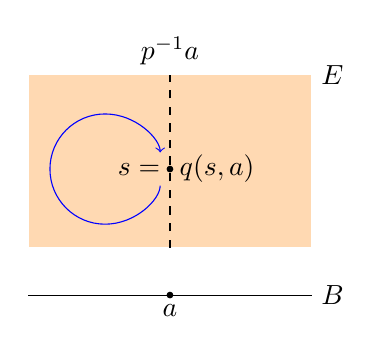
\begin{tikzpicture}

\def\yb{0}; % base
\def\yfb{0.6}; % fiber bottom
\def\yfs{1.1}; % s
\def\yfss{1.6}; % s'
\def\yft{2.8}; % fiber top

\def\dx{0.9};

\def\xbl{0};
\def\xbm{\xbl + \dx};
\def\xbmr{\xbl + 2*\dx};
\def\xbr{\xbl + 4*\dx};


\filldraw[fill=orange!30, draw=white] (\xbl, \yfb) rectangle (\xbr, \yft);

\draw (\xbl, \yb) -- (\xbr, \yb);

\draw[dashed] (\xbmr, \yfb) -- (\xbmr, \yft); %fiber

\node at (\xbmr, \yfss) (s) {};
\draw[->,shorten <=6pt,shorten >=6pt, blue](s.west)arc(360:0:0.7);
\filldraw[black] (\xbmr, \yfss) circle (1 pt);
\node[left] at (\xbmr, \yfss) {$s = $};
\node[right] at (\xbmr, \yfss) {$q(s, a)$};

\filldraw[black] (\xbmr, \yb) circle (1 pt);
\node[below] at (\xbmr, \yb) {$a$};

\node[above] at (\xbmr, \yft) {$p^{-1} a$};
\node[right] at (\xbr, \yb) {$B$};
\node[right] at (\xbr, \yft) {$E$};

\end{tikzpicture}
\]

\subsection{Composition law}

Finally, here's the set/set law, or the \emph{composition} law:
\begin{haskell}
set (set s a) a' = set s a'
\end{haskell}
and the corresponding commuting diagram:
\[
 \begin{tikzcd}
 E \times B \times B
 \arrow[d, "id \times \varepsilon \times id"']
 \arrow[rd, "q \times id"]
 \\
 E \times B
 \arrow[d, "q"']
 & E \times B
 \arrow[dl, "q "]
 \\
 E
  \end{tikzcd}
\]
Again, we use the counit rather than a projection from a product.

This is what the set/set law looks like in a bundle:
\[
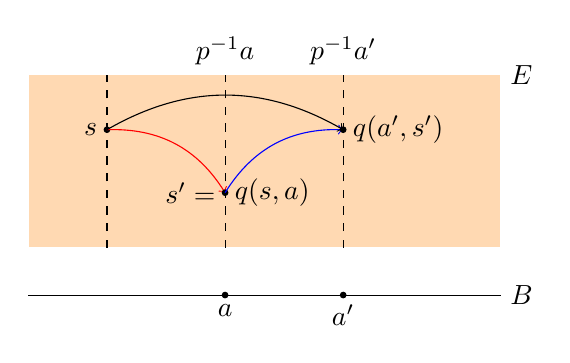
\begin{tikzpicture}

\def\yb{0}; % base
\def\yfb{0.6}; % fiber bottom
\def\yfs{1.3}; % s'
\def\yfss{2.1}; % s''
\def\yft{2.8}; % fiber top

\def\dx{1};

\def\xbl{0};
\def\xbm{\xbl + \dx};
\def\xbmr{\xbl + 2.5*\dx};
\def\xbmrr{\xbl + 4*\dx};
\def\xbr{\xbl + 6*\dx};


\filldraw[fill=orange!30, draw=white] (\xbl, \yfb) rectangle (\xbr, \yft);

\draw (\xbl, \yb) -- (\xbr, \yb);

\draw[dashed] (\xbm, \yfb) -- (\xbm, \yft); %fiber
\draw[dashed] (\xbmr, \yfb) -- (\xbmr, \yft); %fiber
\draw[dashed] (\xbmrr, \yfb) -- (\xbmrr, \yft); %fiber

\filldraw[black] (\xbm, \yfss) circle (1 pt);
\node[left] at (\xbm, \yfss) {$s$};

\draw[red] (\xbm, \yfss)  edge[->, bend left]  (\xbmr, \yfs);

\filldraw[black] (\xbmr, \yfs) circle (1 pt);
\node[right] at (\xbmr, \yfs) {$q(s, a)$};
\node[left] at (\xbmr, \yfs) {$s' =$};

\draw[blue] (\xbmr, \yfs) edge[->, bend left] (\xbmrr, \yfss);

\filldraw[black] (\xbmrr, \yfss) circle (1 pt);
\node[right] at (\xbmrr, \yfss) {$q(a', s')$};

\draw (\xbm, \yfss) edge[->, bend left] (\xbmrr, \yfss);


\filldraw[black] (\xbmr, \yb) circle (1 pt);
\node[below] at (\xbmr, \yb) {$a$};

\filldraw[black] (\xbmrr, \yb) circle (1 pt);
\node[below] at (\xbmrr, \yb) {$a'$};

\node[above] at (\xbmr, \yft) {$p^{-1} a$};
\node[above] at (\xbmrr, \yft) {$p^{-1} a'$};
\node[right] at (\xbr, \yb) {$B$};
\node[right] at (\xbr, \yft) {$E$};

\end{tikzpicture}
\]

\subsection{Type-changing lens}

A type-changing lens generalizes transport to act between bundles. We have to define a whole family of bundles. We start with a category $A$ whose objects define the types that we will use for the foci of our lens. In Haskell, this is the full category of Haskell types. 

We use a set $B$ as the combined set of all elements of all types. $B$ is fibrated over $A$---the projection $\pi$ sending an element of $B$ to its corresponding type. You may think of it as the set of objects of the coslice category $1/A$.

The bundle of bundles $E$ is a set that's fibrated over $B$ with the projection $p$. Since $B$ itself is fibrated over $A$, $E$ is transitively fibrated over $A$, with the composite projection $\pi \circ p$. It's this coarser fibration that splits $E$ into a family of bundles. Each of these bundles represents a different Haskell type. A type-changing lens will move between these bundles.

\[
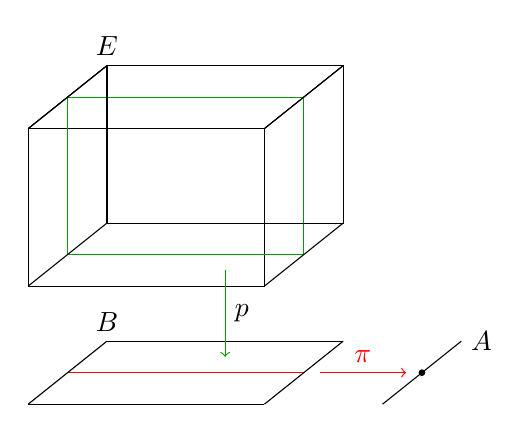
\begin{tikzpicture}
\def\xl{-3};
\def\xr{0};
\def\yb{0};
\def\yt{2};

\def\dy{0.4};
\def\dx{0.5};

\def\a{(\xl, \yb)};
\def\b{(\xr, \yb)};
\def\c{(\xl, \yt)};
\def\d {(\xr, \yt)};

% _a second plane
\def\aa{(\xl + \dx, \yb + \dy)};
\def\ba{(\xr + \dx, \yb + \dy)};
\def\ca{(\xl + \dx, \yt + \dy)};
\def\da{(\xr + \dx, \yt + \dy)};

% _b third plane
\def\ab{(\xl + 2*\dx, \yb + 2*\dy)};
\def\bb{(\xr + 2*\dx, \yb + 2*\dy)};
\def\cb{(\xl + 2*\dx, \yt + 2*\dy)};
\def\db{(\xr + 2*\dx, \yt + 2*\dy)};

% shifted walls
\def\yshift{-1.5};
\def\xshift{1.5};


% E
\draw \a rectangle \d;
\draw[draw=black!40!green] \aa rectangle \da;
\draw \ab rectangle \db;

\draw \a -- \ab;
\draw \b -- \bb;
\draw \d -- \db;
\draw \c -- \cb;

\node[above] at \cb {$E$};

% B
% rebase yb (bottom)
\def\yb{\yshift}
% rebase xr (right wall)
\def\xr{0};

\draw \a -- \b;
\draw \ab -- \bb;
\draw[red] \aa -- \ba;
% diagonal
\draw \a -- \ab;
\draw \b -- \bb;
\draw \d -- \db;
\draw \c -- \cb;
\node[above] at \ab {$B$};


% A
% rebase yb (bottom)
\def\yb{\yshift}
% rebase xr (right wall)
\def\xr{\xshift};

\draw \b -- \bb;
\node[right] at \bb {$A$};
\filldraw[black] \ba circle (1 pt);

%projections

\draw[red, shorten <=0.2cm, shorten >=0.2cm, ->] (0 + \dx, \yshift + \dy) -- node[above]{$\pi$} (\xshift +\dx, \yshift + \dy);

\draw[draw=black!40!green, shorten <=0.2cm, shorten >=0.2cm, ->] (0 - \dx, 0 + \dy) -- node[right]{$p$} (0 - \dx, \yshift + \dy);

\end{tikzpicture}
\]

The projection $p$ takes an element $s \in E$ and produces an element $b \in B$ whose type is given by $\pi b$. This is the generalization of \hask{get}. 

The transport $q$, which corresponds to \hask{set}, takes an element $s \in E$ and an element $b \in B$ and produces a new element $t \in E$. 


The transport satisfies the following laws:

The get/set law (transport):

\[ p (q (b, s)) = b \]

The set/get law (identity):

\[ q ( p (s), s) = s \]

The set/set law (composition):

\[ q (c, q (b, s)) = q (c, s) \]

The two mappings $p$ and $q$ can be combined into one mapping between categories called a \index{cofunctor}cofunctor. 
\section{Important Formulas}
This is a handy (co-)end calculus cheat-sheet.
\begin{itemize}
\item Continuity of the hom-functor:
\[ \mathbf{Set}\left(X, \int_A P\langle A, A \rangle \right) \cong \int_A  \mathbf{Set}(X, P\langle A, A \rangle) \]
\item Co-continuity of the hom-functor:
\[ \mathbf{Set}\left( \int^A P\langle A, A \rangle , X\right) \cong \int_A  \mathbf{Set}(P\langle A, A \rangle, X) \]
\item Ninja Yoneda:
\[ \int_{X} \mathbf{Set} (\mathcal{C}(A, X), FX) \cong FA \]
\item Ninja co-Yoneda:
\[ \int^{X} \mathcal{C}(X, A) \times F X \cong F A \]
\item Ninja Yoneda for contravariant functors (pre-sheaves):
\[ \int_{X} \mathbf{Set} (\mathcal{C}(X, A), GX) \cong GA \]
\item Ninja co-Yoneda for contravariant functors:
\[ \int^{X} \mathcal{C}(A, X) \times G X \cong G A \]
\end{itemize}


\end{document}